% FIG:q19-cuboid
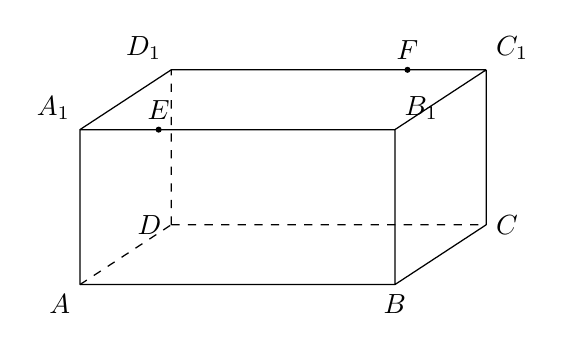
\begin{tikzpicture}[x={(1cm,0cm)},y={(0.58cm,0.38cm)},z={(0cm,0.82cm)},line width=0.45pt]
  \coordinate (A) at (0,0,0);
  \coordinate (B) at (4,0,0);
  \coordinate (C) at (4,2,0);
  \coordinate (D) at (0,2,0);
  \coordinate (Aone) at (0,0,2.4);
  \coordinate (Bone) at (4,0,2.4);
  \coordinate (Cone) at (4,2,2.4);
  \coordinate (Done) at (0,2,2.4);
  \coordinate (E) at (1,0,2.4);
  \coordinate (F) at (3,2,2.4);
  \draw (A)--(B)--(C) (A)--(Aone)--(Bone)--(B) (Bone)--(Cone) (Cone)--(C)
    (Aone)--(Done)--(Cone) (Done)--(F) (Aone)--(E);
  \draw[dashed] (A)--(D) (D)--(C) (D)--(Done);
  \foreach \p/\pos/\lab in {A/below left/A,B/below/B,C/right/C,D/left/D,Aone/above left/{A_1},Bone/above right/{B_1},Cone/above right/{C_1},Done/above left/{D_1},E/above/{E},F/above/{F}} {
    \node[\pos] at (\p) {$\lab$};
  }
  \fill (E) circle (1.1pt);
  \fill (F) circle (1.1pt);
\end{tikzpicture}
